% Opcje klasy 'iithesis' opisane sa w komentarzach w pliku klasy. Za ich pomoca
% ustawia sie przede wszystkim jezyk oraz rodzaj (lic/inz/mgr) pracy.
\documentclass[shortabstract]{iithesis}

\usepackage[utf8]{inputenc}
\usepackage{hyperref}
\usepackage{graphicx}
\usepackage{paralist}
\usepackage{listings}

% \usepackage{tikz}
% \usepackage{pgfplots}
% \usepackage[simplified]{pgf-umlcd}
% \pgfplotsset{compat=1.18}

%%%%% DANE DO STRONY TYTUŁOWEJ
% Niezaleznie od jezyka pracy wybranego w opcjach klasy, tytul i streszczenie
% pracy nalezy podac zarowno w jezyku polskim, jak i angielskim.
% Pamietaj o madrym (zgodnym z logicznym rozbiorem zdania oraz estetyka) recznym
% zlamaniu wierszy w temacie pracy, zwlaszcza tego w jezyku pracy. Uzyj do tego
% polecenia \fmlinebreak.
\polishtitle    {Aplikacja mobilna do zarządzania i tworzenia\fmlinebreak  interaktywnych notatek}
\englishtitle   {A mobile application to manage and create interactive notes}
\polishabstract {TODO: streszczenie po polsku\ldots}
\englishabstract{TODO: streszczenie po angielsku\ldots}
% w pracach wielu autorow nazwiska mozna oddzielic poleceniem \and
\author         {Bartosz Sobocki}
% w przypadku kilku promotorow, lub koniecznosci podania ich afiliacji, linie
% w ponizszym poleceniu mozna zlamac poleceniem \fmlinebreak
\advisor        {dr Marcin Młotkowski}
%\date          {}                     % Data zlozenia pracy
% Dane do oswiadczenia o autorskim wykonaniu
%\transcriptnum {}                     % Numer indeksu
%\advisorgen    {dr. Marcina Młotkowskiego} % Nazwisko promotora w dopelniaczu
%%%%%

%%%%% WLASNE DODATKOWE PAKIETY
%
%\usepackage{graphicx,listings,amsmath,amssymb,amsthm,amsfonts,tikz}
%
%%%%% WŁASNE DEFINICJE I POLECENIA
%
%\theoremstyle{definition} \newtheorem{definition}{Definition}[chapter]
%\theoremstyle{remark} \newtheorem{remark}[definition]{Observation}
%\theoremstyle{plain} \newtheorem{theorem}[definition]{Theorem}
%\theoremstyle{plain} \newtheorem{lemma}[definition]{Lemma}
%\renewcommand \qedsymbol {\ensuremath{\square}}
% ...
%%%%%

\begin{document}

%%%%% POCZĄTEK ZASADNICZEGO TEKSTU PRACY

\chapter{Wprowadzenie}

\section{Cel projektu}

Celem projektu jest wytworzenie aplikacji mobilnej do zarządzania notatkami w interaktywny sposób.
Aplikacja ma umożliwić użytkownikowi prowadzenie i tworzenie notatek pozwalających na formatowanie tekstu i dołączanie załączników.
Formatowanie tekstu wzorowane będzie na języku znaczników Markdown. Główną różnicą w stosunku do edytorów używających tego typu formatowania tekstu będą:
\begin{compactitem}
    \item brak konieczności zmian widoków (pomiędzy edycją surowego tekstu, a widokiem zawierającym sformatowany tekst);
    \item przełączenia całej zawartości pomiędzy trybem edycji, a trybem użytkowym;
    \item potrzeby zapisu notatki do wyświetlania formatowania i zawartych załączników.
\end{compactitem}

Graficzny interfejs użytkownika powinien być przystępny i pozwalać na formatowanie wybranych elementów, podczas gdy pozostała zawartość notatki jest wyświetlana w trybie widoku.
Do przechowywania zawartości notatek powinna zostać użyta baza danych, jak również odpowiedni format zapisu danych do przechowywania zawartości niebędącej tekstem.

\section{Motywacja}

Motywacją do stworzenia projektu MobiNote była potrzeba aplikacji pełniącej rolę brudnopisu używanego podczas wielu codziennych czynności. Jestem osobą, która uwielbia:

\begin{compactitem}
    \item tworzyć notatki;
    \item prowadzić dzienniki;
    \item zapisywać przepisy;
    \item tworzyć wszelakie listy;
    \item dzielić problemy na mniejsze części i rozpisywać je;
    \item  prowadzić różnego rodzaju zeszyty.
\end{compactitem}
Dzięki temu mogę zawsze sięgać do zapisków swoich myśli i pomysłów w chwilach, gdy są mi potrzebne.

Dostępne na rynku aplikacje, takie jak Evernote, czy ostatnio używane przeze mnie proste w użyciu Samsung Notes, w wielu aspektach sprawdziło się i przyniosło wiele korzyści. W obu przypadkach interfejs użytkownika jest przejrzysty, a funkcjonalność obszerna. Jednak po dłuższym okresie użytkowania tych, oraz innych aplikacji dostrzegam w nich problemy lub braki, dlatego chciałbym używać notatnika wolnego od nich.

Bardzo lubię korzystać z języka znaczników Markdown. Oferuje on możliwość formatowania tekstu, tworzenia różnych nagłówków i elementów notatki przy użyciu jedynie odpowiedniej składni zawartej w zwykłym tekście. W przeciwieństwie do omawianych wyżej aplikacji nie trzeba:
\begin{compactitem}
    \item przeszukiwania opcji w poszukiwaniu przycisków, którymi użytkownik określa typ i wielkość czcionki;
    \item przełączania zwkłej klawiatury na klawiaturę zawierającą narzędzia do formatowania tekstu;
    \item wchodzenia w menu aby zaimportować zdjęcia, dodać listy itd.
\end{compactitem} 
Używanym przeze mnie serwisem był \textbf{HackMD}. Dużym minusem jednak był brak aplikacji mobilnej, oraz dwa ekrany: edycji tekstu i wygenerowanej notatki. Zależało mi na tym, aby notatka była renderowana i formatowana na bieżąco na jednym ekranie z ewentualnym ujawnianiem i chowaniem znaczników w tekście. Tekst powinien być stylizowany już w polu tekstowym uwzględniając dodawanie i usuwanie znaczników w czasie rzeczywistym.

Chciałem stworzyć aplikację, która będzie posiadała szereg wymaganej przeze mnie funkcjonalności, jak na przykład:
\begin{compactitem}
    \item liczniki, abym mógł w trakcie treningu odliczać wykonane serie;
    \item alarmów, które odliczałyby przerwy pomiędzy seriami;
    \item przycisków informacyjnych otwierających okno dialogowe z informacjami dotyczącymi na przykład wymienionego w notatce miejsca;
    \item edycji stylów tekstu za pomocą znaczników, zamiast przycisków i odrębnej klawiatury. 
\end{compactitem}
Aplikacja nie powinna wymagać ode mnie dużego wysiłku podczas tworzenia zapisków: 
\begin{compactitem}
    \item pracując nad projektem;
    \item ucząc się nowych rzeczy;
    \item zapisując myśli w nocy tuż przed spaniem.
\end{compactitem}
Chciałem, aby aplikacja była szybka, prosta i przejrzysta, jednocześnie pozwalając użytkownikowi na dodawanie, edycję oraz interakcję różnego typu widgetów, alarmów czy powiadomień. Wtedy aplikacja może również służyć w stanie, gdy aktualnie nie jest edytowana. W moich intencjach było, aby interfejs użytkownika był dopasowany do moich potrzeb i gustu. Chciałem, by aplikacja odpowiadała mi pod wieloma względami, nie tylko w kwestii oferowanych funkcji, ale również wyglądu, czy rozmieszczenia i dostępności funkcji, przycisków, czy widgetów tak, aby te najczęściej używane były najłatwiej dostępne i proste w obsłudze.

\section{Opis aplikacji MobiNote}

Aplikacja MobiNote służy do tworzenia i zarządzania notatkami w sposób opisany powyżej.
Głównym zamysłem aplikacji jest pomoc korzystającemu w prowadzeniu, tworzeniu i zapisywaniu notatek, w których skład wchodzi nie tylko tekst, ale również przyciski, obrazy, listy, liczniki i różnego rodzaju pomocne widgety.
Aplikacja umożliwia tworzenie i utrzymywanie brudnopisu używanego podczas codziennych czynności, jak również przejrzystych, dopracowanych i przystępnych  notatek.

Wytworzone notatki mogą być używane w formie brudnopisu, między innymi podczas:
\begin{compactitem}
    \item treningu na siłowni;
    \item organizacji przyjęcia;
    \item nauki z wykorzystaniem sesji pomodoro;
    \item tworzeniu listy zakupów;
    \item wielu innych codziennych czynności.
\end{compactitem}

Mogą także w przyjemny dla oka sposób przechowywać i wyświetlać informacje przygotowane w celu tworzenia:
\begin{compactitem}
 \item dziennika;
 \item notatek do nauki;
 \item spisu pomysłów i ważnych myśli;
 \item różnego rodzaju list i opisów.
\end{compactitem}
 Przykładem może być lista miejsc, które użytkownik chciałby odwiedzić wraz z opisem i zdjęciami miejsc, które chciałby tam zobaczyć.

Interaktywność notatki jest zapewniana poprzez możliwość tworzenia zawartości na bieżąco za pomocą klawiatury i dostępnego interfejsu użytkownika.
Użytkownik może tworzyć styl tekstu za pomocą znaczników dodawanych wewnątrz tekstu w odpowiednich miejscach, podobnie do języka znaczników Markdown.
Dodając odpowiednie znaczniki w tekście można ustawić wielkość czcionki w danym akapicie, kursywę, podkreślenie, przekreślenie, a także pogrubienie.
Tekst jest automatycznie formatowany wraz z dodaniem znaczników, co pozawala na bieżąco obserwować i dostosowywać style i wielkości czcionki do potrzeb korzystającego.

Notatki będą zapisywane lokalnie, co pozwoli zaoszczędzić czas ładowania, jak również pominąć problemy związane z synchronizacją.

Interfejs użytkownika jest prosty i przejrzysty, posiada motyw ciemny (\textbf{dark}), jasny (\textbf{light}) oraz ułatwiający użytkowanie (\textbf{easy}) dla osób słabowidzących.

\chapter{Instalacja}

Aplikacja MobiNote jest dostępna i testowana na urządzeniach android.
Kod żródłowy aplikacji wraz z plikiem \textbf{.apk} można uzyskać pobierając repozytorium \textbf{MobiNote} pod linkiem:
\url{https://github.com/bsobocki/MobiNote}.

\section{Android}

 Do instalowania aplikacji na urządzeniach posiadających system Android, Google wprowadziło platformę \textbf{Google Play}. Oferuje ona możliwości sprawdzenia aplikacji pod względem niechcianych zachowań, czy instalacji złośliwego oprogramowania. Aplikacje są instalowane za pomocą dostępnego interfejsu użytkownika. Domyślne ustawienia urządzenia pozwalają wyłącznie na instalacje aplikacji z zaufanego źródła, jakim jest wspomniany \textbf{Google Play} \cite{googleplay}.

Istnieje również niestandardowy sposób instalacji aplikacji bez użycia oferowanego rozwiązania opisanego powyżej. Użytkownik może zainstalować aplikację za pośrednictwem pliku o rozszerzeniu \textbf{.apk}. Użytkownik robi to na własną odpowiedzialność, dlatego ważne, żeby aplikacja pochodziła z zaufanego źródła. Aby to zrobić, należy wyłączyć blokadę instalacji aplikacji z nieznanych źródeł.

\subsection{Instalacja aplikacji z nieznanych źródeł}
Do zainstalowania aplikacji MobiNote potrzebna jest wyłączona blokada instalacji aplikacji z nieznanych źródeł dla menadżera plików.
W tym celu należy:
\begin{compactitem}
    \item otworzyć \textbf{Ustawienia}
    \item w \textbf{Ustawieniach} przejść do sekcji \textbf{Aplikacje}
    \item następnie kliknąć na ikonę menu (trzy kropki w prawym górnym rogu)
    \item przejść do opcji \textbf{Dostęp specjalny}
    \item następnie \textbf{Zainstaluj nieznane aplikacje}
    \item wybrać menadżera plików i włączyć dla niego tę opcję
\end{compactitem}

\textbf{Ważne!} Dla bezpieczeństwa po zainstalowaniu aplikacji warto ponownie wyłączyć możliwość instalowania aplikacji z nieznanych źródeł, jeśli więcej aplikacji nie będzie w ten sposób instalowanych.

\subsection{Instalacja z pliku apk-release.apk}

Aby zainstalować aplikację na urządzeniu mobilnym z systemem Android należy:
\begin{compactitem}
    \setlength\itemsep{0mm}
    \item pobrać repozytorium za pomocą polecenia
    \newline
    \verb|git clone git@github.com:bsobocki/MobiNote.git|
    \item podłączyć urządzenie i przenieść pliki \textbf{apk-release.apk} do wybranego przez siebie miejsca docelowego na urządzeniu;
    \item włączyć możliwość instalacji nieznanych aplikacji (szczegóły powyżej);
    \item w managerze plików znaleźć miejsce docelowe pliku \textbf{apk-release.apk} i uruchomić;
    \item kliknąć \textbf{Zainstaluj}.
\end{compactitem}

\chapter{Podręcznik Użytkownika}
\label{ch:manual}

\section{Strona Domowa}

Po uruchomieniu aplikacji użytkownik zostaje przeniesiony na stronę domową. Znajdzie tam swoje notatki i zeszyty wraz z przyciskiem w prawym dolnym rogu służącym do tworzenia nowej notatki, jak również dodatkowe elementy w menu górnego paska, pozwalające na zmianę motywu, czy reset bazy danych w celu usunięcia wszystkich notatek. 

\begin{figure}[ht]
    \centering
    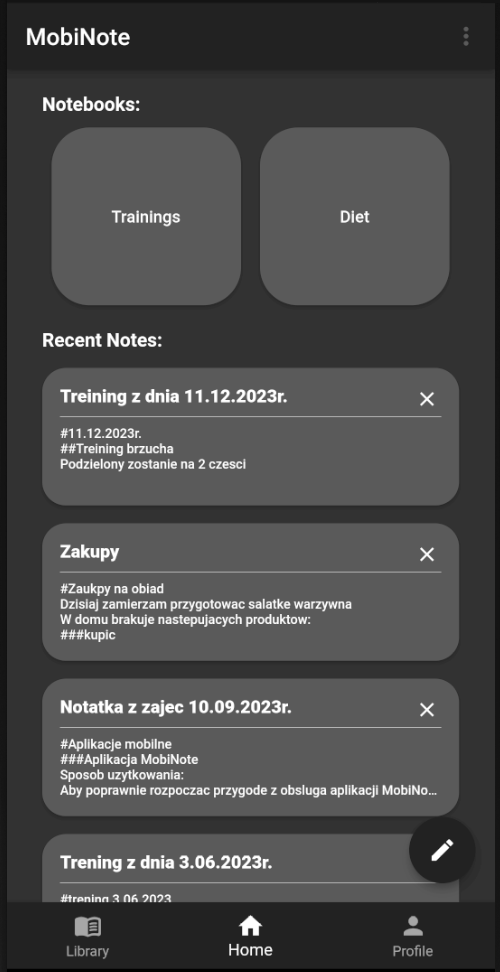
\includegraphics[height=10cm]{images/strona_domowa.png}
    \quad\quad
    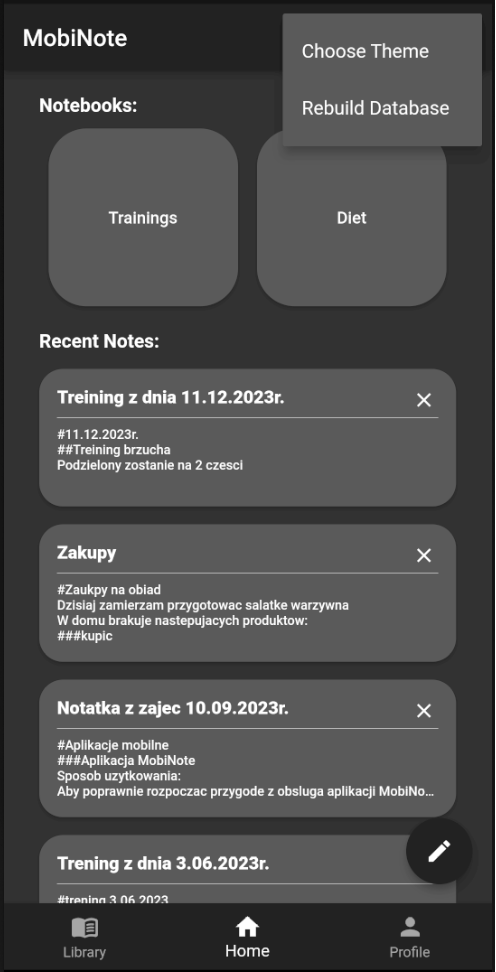
\includegraphics[height=10cm]{images/strona_domowa_opcje.png}
    \caption{Strona domowa aplikacji MobiNote z wybranym motywem \textbf{dark}.}
\end{figure}

\subsection{Opcja \textit{Choose Theme}}

Po uruchomieniu tej opcji wyświetli się okienko dialogowe z wyborem motywu, jakiego użytkownik chciałby użyć. Do wyboru mamy trzy mowtywy: \textbf{dark}, \textbf{light} oraz \textbf{easy}.

Motywy \textbf{dark} oraz \textbf{light} służą, jako główne motywy aplikacji, zachowując te same wielkości elementów tekstu i całej aplikacji.
Dla osób mających problemy z widocznością tekstu przy domyślnych ustawieniach wielkości i kolorów aplikacji przygotowany został mowtyw \textbf{easy}.
Motyw ten cechują kontrastujące ze sobą kolory, jak również zwiększone rozmiary czcionek, ikon, przycisków i paska narzędzi.

\begin{figure}[ht]
    \centering
    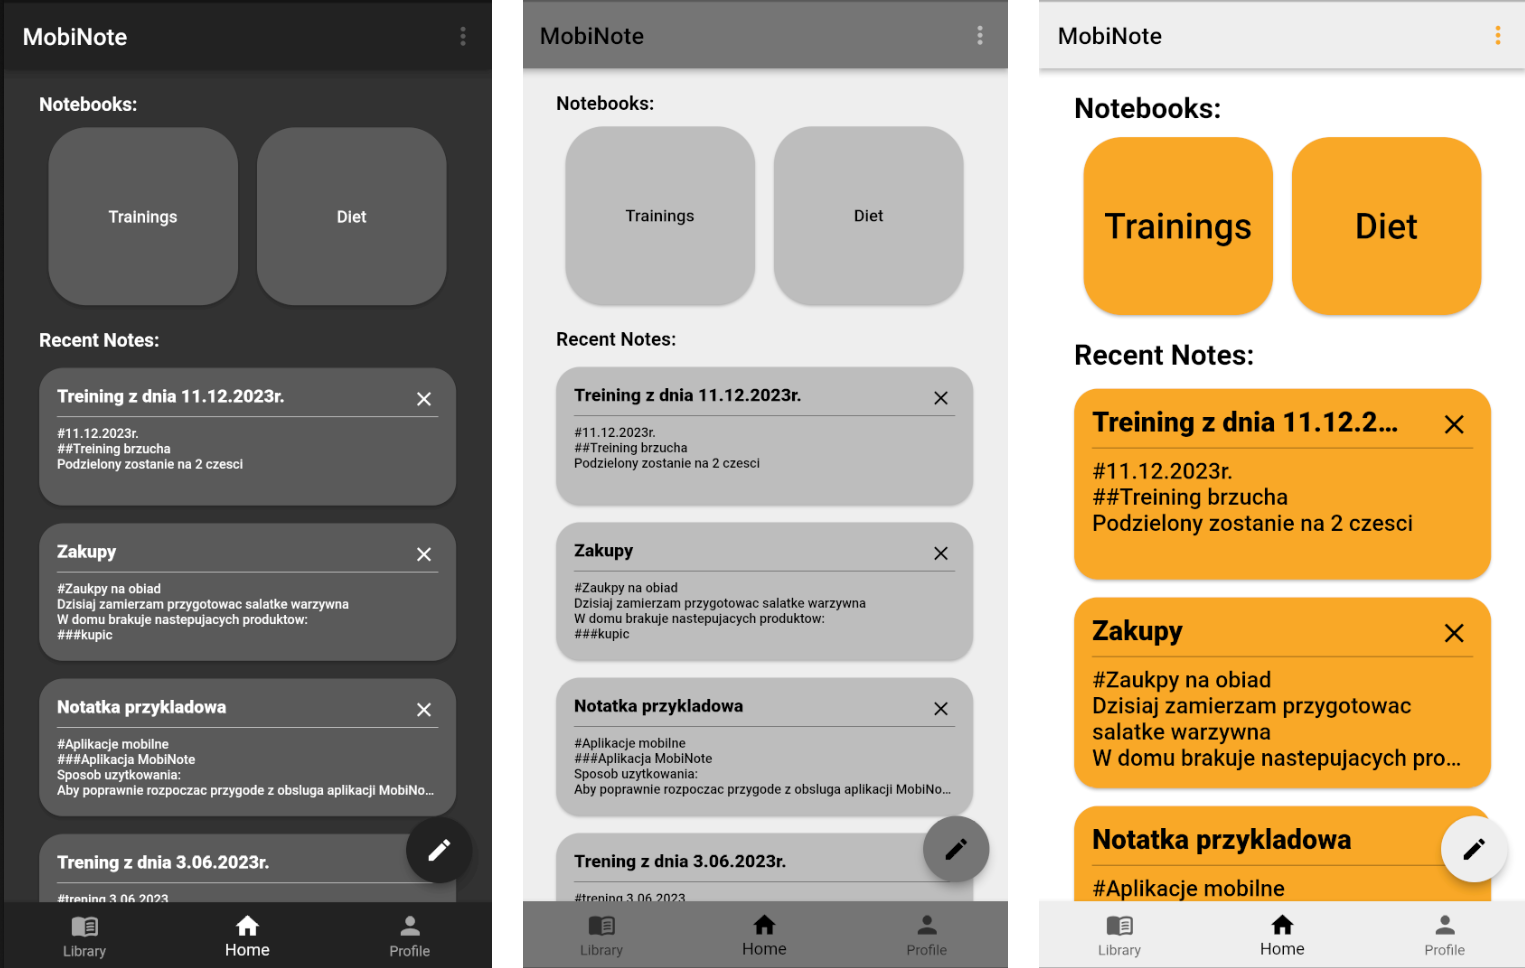
\includegraphics[height=8.5cm]{images/strona_domowa_motywy.png}
    \caption{Porównanie motywów na tej samej stronie domowej.}
\end{figure}

\subsection{Opcja \textit{Rebuild Database}}

Opcja ta otwiera okno dialogowe z pytaniem o to, czy na pewno chcemy wykonać tę przebudowanie bazy danych. Po zatwierdzeniu baza danych jest usuwana i budowana.

\subsection{Zeszyty}

Pod etykietą \textbf{\textit{Notebooks:}} widnieją dwa przyciski \textbf{Trainings} oraz \textbf{Diet}. Są to roboczo dodane przyciski, które są przygotowane pod rozszerzenie aplikacji w przyszłości o możliwość układania notatek w zeszyty, dla lepszej organizacji, a także wprowadzać etykiety.
Pomysł ten zostanie omówiony w rozdziale \textbf{Rozszerzenie Funkcjonalnosći aplikacji}.

\subsection{Notatki}

Kolejnym elementem strony domowej jest lista notatek znajdująca się pod etykietą \textbf{\textit{Recent Notes:}}. Każdy element zawiera tytuł oraz pierwsze cztery surowe linie tekstu(zawierające znaki specjalne styli w przypadku paragrafu będącego tekstem, lub string w formacie JSON reprezentujący widget zawarty w danym paragrafie).
W prawym górnym rogu elementów znajduje się przycisk \textbf{X} służący do usunięcia danej notatki z bazy danych.
Po naciśnięciu na dany element użytkownik zostaje przeniesiony do ekranu wyświetlania i edycji wybranej notatki.

W prawym dolnym rogu ekranu widnieje okrągły przycisk z ikoną ołówka.
Po jego naciśnięciu korzystający zostaje przeniesiony do ekranu edycji, gdzie może stworzyć i zapisać nową notatkę.

\section{Strona Edycji Notatki}

Po wybraniu notatki, lub przejściu do tworzenia nowej, na ekranie pojawi się strona edycji notatki. Składa się ona z głównego paska strony, paska narzędzi, oraz edytora.
\subsection{Pasek Strony}

\subsubsection{Przycisk Zapisu i Powrotu}

Aby wyjść i zapisać notatkę korzystający używa przycisku powrotu.
Ważnym jest, aby zamiast systemowych przycisków nawigacyjnych użyć właśnie tego przycisku nawigacyjnego, ponieważ wraz z powrotem do strony domowej zapisuje on notatkę, jeśli ta uległa zmianie.

Za zmianę notatki unawane są:

\begin{compactitem}
    \item edycja tekstu w paragrafie tekstowym
    \item edycja widgetu w paragrafie widgetu
\end{compactitem}
\vspace{5mm}

\textbf{WAŻNE!} Nowa notatka nie zostaje utworzona w momencie otwarcia okna edycji, a dopiero poprzez użycie przycisku powrotu pod warunkiem, ze jej tytuł lub zawartość uległy edycji. Oznacza to, że przejście do edycji nowej notatki, a następnie powrót, nie zapiszą pustej notatki, jednak dodanie i usunięcie znaku umożliwią zapis przy powrocie.

\subsubsection{Edytor tytułu}

Jest to pole tekstowe widniejące zaraz obok \textbf{Przycisku zapisu i powrotu}. Służy ono do edycji tytułu notatki.

\subsubsection{Przycisk zmiany opcji zapisu}

Ostatnim elementem paska jest \textbf{przycisk zmiany opcji zapisu}. Jest to przycisk typu \textbf{switch} domyślnie ustawiony na true. Każdorazowe kliknięcie zmienia jego logiczną wartość.
Wartość \textbf{true} oznacza zapis notatki w przypadku jej edycji, natomiast \textbf{false} oznacza brak zapisu stanu notatki, nawet jeśli została ona zmieniona.

\subsection{Pasek Narzędzi}

W tym pasku znajdują się przyciski oznaczone ikonami.
W aktualnej wersji aplikacji dostępne są dwa przyciski: dodanie obrazu(ikona obrazu), oraz dodanie listy(ikona listy).

\subsubsection{Dodanie obrazu}

Do zawartości notatki można dodawać również obrazy. Aby to zrobić należy kliknąć przycisk z ikoną obrazu na pasku narzędzi edytora notatki, a następnie wybrać z urządzenia zdjęcie, które ma zostać użyte. Zdjęcie zostanie dodane do notatki.

\subsubsection{Dodanie listy}

Po wybraniu tej opcji na ekranie pojawi się lista złożona początkowo z jednego elementu.
Jest on domyślnie ustwawiony na typ \textbf{checkbox}. Oznacza to, że jest to wiersz zawierający checkbox oraz puste pole tekstowe.

\subsection{Edytor Strony}

Edytor strony zajmuje reszę powierzchni ekranu. Jest polem, w którym następuje edycja tekstu oraz widgetów. Aktualny stan wizualny jest odświeżany na bieżąco, dzięki czemu użytkownik obserwuje zmiany jako efekt końcowy w czasie rzeczywistym.



\section{Edycja Zawartości Notatki}

\subsection{Paragrafy}

Notatki w aplikacji składają się z paragrafów, które dzielimy na paragrafy tekstowe i paragrafy widgetów.
Każdy paragraf może przechodzić w jedne z dostępnych trybów.
Obecnie wyróżnione są tryby:

\begin{compactitem}
    \item widoku
    \item edycji
    \item zaznaczenia
    \item niewidoczny
\end{compactitem}

\subsubsection{tryb widoku}

Paragraf istnieje w trybie widoku, kiedy nie jest aktywny.
Paragraf przechodzi w tryb widoku, w momencie przeniesienia aktywności na inny paragraf(na przykład poprzez kliknięcie).

\subsubsection{tryb edycji}

Paragraf przechodzi w tryb edycji, w momencie przeniesienia na niego aktywności.
Aktywność ta może zostać przeniesiona poprzez kliknięcie na elementy paragrafu, lub w przypadku, gdy jest to paragraf widgetów, a jego następnikiem jest paragraf tekstowy, którego edytujący stara się usunąć.

\subsubsection{tryb zanzaczenia}

Paragraf widgetów przechodzi w tryb zaznaczenia poprzez przytrzymanie jego elementów niebędących polem tekstowym(poniważ pole tekstowe ma już zarezerwowany ten gest na zaznaczanie tekstu).

\subsubsection{tryb niewidoczny}

Paragraf przestaje być widoczny w momencie przejścia edytora w kierunku pionowym wystarczająco do wysunięcia paragrafu poza edytor.

\pagebreak

\subsection{Edycja Paragrafów Tekstowych}

Każdy tekst zamykany jest w paragrafie tekstowym od początku, aż do znaku końca linii. Oznacza to, że styl, jaki zostanie nadany na początku linii zostanie zaaplikowany na całą linię. Przykładem jest ustawienie paragrafu jako nagłówka.

\subsubsection{Dodawanie}

Dodawanie paragrafów tekstowych odbywa się za pomocą klawiatury. W momencie, gdy użytkownik podczas edycji doda znak nowej linii, wówczas utworzy się nowy paragraf, będący następnikiem edytowanego.

\textbf{Ważne:} Podczas dodawania nowego paragrafu widgetów utworzy się nowy paragraf tekstowy jako jego następnik. Ma to na celu zachowanie możliwości ciągłej pracy z tekstem.

\subsubsection{Usuwanie}

Usunąć paragraf tekstowy można poprzez naciśnięcie przycisku \textbf{delete} na samym początku tekstu. Jeśli poprzedni paragraf jest paragrafem tekstowym, wówczas pozostały tekst kopiowany jest na koniec poprzedniego paragrafu.

\subsubsection{Ustawianie nagłówka}

Ustawienie nagłówka odbywa się poprzez wstawienie znaku \textbf{\#} na początku linii, przed tekstem.

\subsubsection{Dostępne nagłówki}
\begin{itemize}
    \setlength\itemsep{0mm}
    \item nagłówek1 \textbf{\#}
    \item nagłówek2 \textbf{\#\#}
    \item nagłówek3 \textbf{\#\#\#}
    \item nagłówek4 \textbf{\#\#\#\#}
\end{itemize}

Brak nagłówka oznacza, że dana linia jest zwykłym paragrafem o domyślnej wielkości czcionki i odstępów oraz nie zawiera pogrubienia.

\pagebreak

\subsubsection{Odkrywanie znaków nagłówka}

Edytor posiada funcję odkrywania znaków nagłówka, w celu ułatwienia edycji danego nagłówka. Dzięki temu użytkownik może zobaczyć który aktualnie nagłówek jest wybrany oraz w prosty sposób przechodzić pomiędzy typami nagłówków dodając bądź usuwając znak \textbf{\#}.


\begin{figure}[ht]
    \centering
    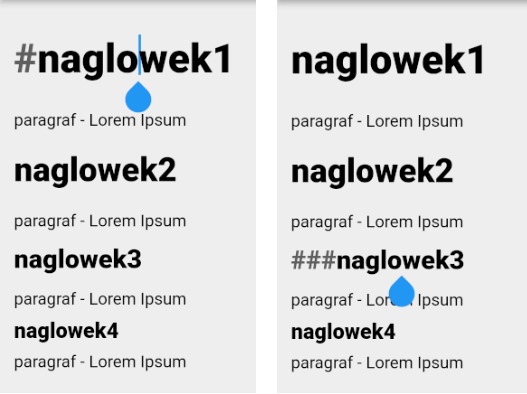
\includegraphics[height=6cm]{images/pokazywanie_naglowkow.png}
    \caption{Odkryte znaki w edytowanych nagłówkach.}
\end{figure}

\subsubsection{Ustawianie styli}

Kolejną rzeczą dostępną w aplikacji MobiNote są style. Użytkownik, chcąc poprawnie nadać style, wprowadza do tekstu symbole specjalne oznaczające konkretne style.
Odbywa się to według poniższych zasad:

\begin{itemize}
    \setlength\itemsep{2mm}

    \item za początek oznaczenia stylu uznawany jest wzór: \newline
    \verb|[dowolny znak][symbol stylu][znak niebędący białym znakiem]|
    
    \item za koniec oznaczenia stylu uznawany jest wzór: \newline
    \verb|[znak niebędący białym znakiem][symbol stylu]|
    
    \item style mogą być łączone -- wewnątrz stylu A można dodać styl B

    \item style nie mogą być krzyżowane -- jeśli zaczynamy styl B wewnątrz stylu A, to znak końca stylu B powinien nastąpić przed symbolem końca A. 
\end{itemize}

\begin{figure}[ht]
    \centering
    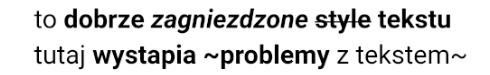
\includegraphics[width=8cm]{images/style.png}
    \caption{Zagnieżdżone style w prawidłowy i nieprawidłowy sposób}
    \vspace{3mm}
\end{figure}

\begin{figure}[ht]
    \centering
    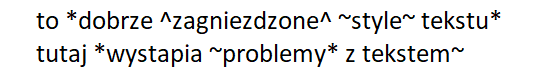
\includegraphics[width=8cm]{images/style_surowy_tekst.png}
    \caption{Surowy tekst ukazujący rozmieszczenie znaków.}
    \vspace{3mm}
\end{figure}

\subsubsection{Znaki specjalne}

Każdy dostępny styl tekstu oznaczony jest za pomocą znaków:

\begin{compactitem}
    
    \item [*] \hspace{1mm} -- pogrubienie
    \item [\^{}] \hspace{1mm} -- kursywa
    \item [\_{}] \hspace{1mm} -- podkreślenie
    \item [\~{}] \hspace{1mm} -- przekreślenie
\end{compactitem}

\subsubsection{Odkrywanie znakow specjalnych}

Edytor tekstu posiada funkcję odwijania stylu w moemncie gdy kursor znajduje się bezpośrednio w środku stylu. Odwijany jest tylko styl, którego jeden ze znaków specjalnych znajduje się najbliżej kursora. Funkcjonalność ta została wprowadzona, aby użytkownik mógł łątwiej edytować i usuwać style.
Dzięki temu może dostrzec, gdzie konkretnie znajdują się symbole danego stylu w tekście.


\begin{figure}[ht]
    \centering
    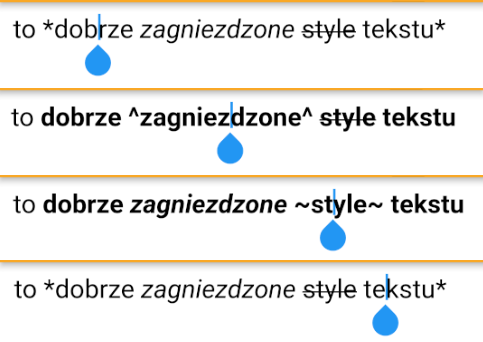
\includegraphics[width=8cm]{images/pokazywanie_znakow_specjalnych.png}
    \caption{Przykłady odkrytych znaków specjalnych.}
    \vspace{3mm}
\end{figure}

\subsubsection{Usuwanie i Edycja styli}

Aby usunąć dany styl wystarczy usunąć znaki specjalne danego stylu. Poza odkrytymi znakami reszta jest ukryta, jednak wszystkie znaki nadal występują w tekście. Edytujący może zatem kliknąć bespośrednio przed widoczny początkowy symbol lub poza tekst oznaczony danym stylem i naciskając przycisk \textbf{delete}, na klawiaturze urządzenia, usunąć dany niewidoczny symbol zakończenia stylu.

\pagebreak

\subsection{Edycja Paragrafów Widgetów}

Elementami tych paragrafów są widgety. W aktualnej wersji aplikacji dostępne są dwa widgety, które mogą być bezpośrednimi elementami paragrafów widgetów.
Są to \textbf{obrazy} i \textbf{listy}.

\subsubsection{Dodawanie}

Dodawanie paragrafów widgetów odbywa się poprzez użycie przycisków z paska narzędzi edytora notatki.

\subsubsection{Usuwanie}

Usunąć paragraf widgetów można poprzez usunięcie jego wszsytkich głównych elementów. W obecnej wersji możliwe jest posiadanie tylko jednego głównego elementu, jednak przewidziane w rozwoju aplikacji jest, aby paragrafy mogły przechowywać i używać większej ilości widgetów, w zależności od rodzajów używanych widgetów.

\subsubsection{Tryb Edycji}

Przejście do trybu edycji odbywa się poprzez interakcję z widgetem, np naciśnięcie na obraz, bądź edycja tekstu w elemencie listy.
W przypadku obrazów tryb edycji jest oznaczony poprzez dodanie obramowania do zdjęcia, jak również ikony w dolnej części obramowania służącej do zmiany rozmiaru zdjęcia.

\begin{figure}[ht]
    \centering
    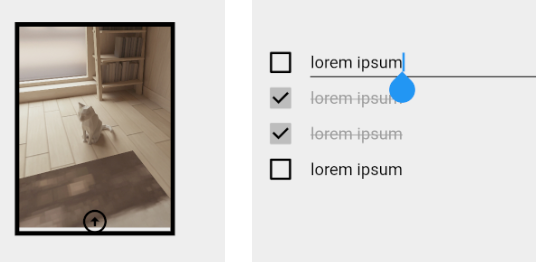
\includegraphics[width=6cm]{images/tryb_edycji.png}
    \caption{Tryb edycji przykładowych widgetów głównych.}
    \vspace{3mm}
\end{figure}

\subsubsection{Tryb zaznaczenia}

Przejście w tryb zaznaczenie odbywa się poprzez naciśnięcie i przytrzymanie konkretnych części widgetów. W przypadku obrazu jest to sam obraz, z kolei w przypadku list są to etykiety przypięte do pola tekstowego(w zależności od wyboru mogą być to: checkbox, etykiety tekstowe czy liczniki).

\begin{figure}[ht]
    \centering
    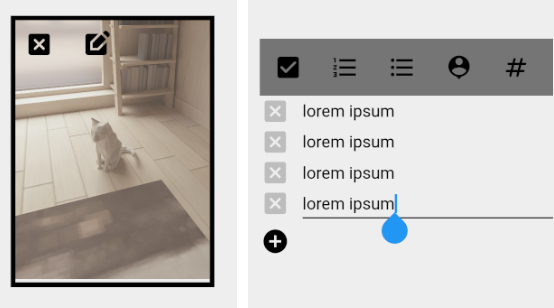
\includegraphics[width=6cm]{images/tryb_zaznaczenia.png}
    \caption{Tryb zaznaczenia przykładowych widgetów głównych.}
    \vspace{3mm}
\end{figure}


\subsection{Obrazy}

Jednym z głównych widgetów są obrazy. 

Dodawane są poprzez użycie przycisku na pasku narzędzi(sekcja: Pasek Narzędzi: Dodanie obrazu). Obraz wybierany jest z pamięci urządzenia.

\subsubsection{Edycja}

Aby zmienić rozmiar zdjęcia użytkownik musi przejść w tryb edycji poprzez kliknięcie na zdjęcie, a następnie przeciągać ikonę ze strzałką(Rysunek 3.8). Automatycznie dostosowywany będzie rozmiar obrazu.

\subsubsection{Usunięcie i zmiana}

Po wejściu w tryb zaznaczenia ukażą się dwie ikony. Ikona usunięcia obrazu oraz ikona zmiany obrazu.
Wybór pierwszej ikony skutkuje usunięciem obrazu wraz z paragrafem, natomiast drugiej -- przejściem do pamięci urządzenia w celu wyboru zdjęcia.

\subsection{Listy}

Dostępne są różne rodzaje list. Różnią sie one głównie etykietą oraz niewielkimi kwestiami, jak na przykład dostępne przekreślenie i zmiana koloru tekstu przy odznaczonej pozycji.

\subsubsection{Edycja}

Edycja list następuje poprzez interakcję użytkownika. Użytkownik może naciskać bezpośrednio na etykiety przy polu tekstowym w celu ich edycji(checkbox, licznik), jak również edytować tekst wiersza.

W przypadku niektórych typów wiersza możliwe jest jego odznaczenie. Wówczas tekst wiersza zmienia kolor na szary, a sam tekst zostaje przekreślony.

\subsubsection{Dodawanie wierszy}

Dodawanie wierszy następuje na dwa sposoby:

\begin{enumerate}
    \item W dowolnym miejscu listy poprzez dodanie znaku nowej linii.
    \item Na koniec listy poprzez kliknięcie przycisku "+" pod etykietami w trybie zaznaczenia. 
\end{enumerate}

Dodawanie wierszy poprzez znak nowej linii przenosi tekst na prawo od miejsca dodania znaku nowej linii do nowego wiersza.

\subsubsection{Usuwanie wierszy}

Usuwanie wierszy jest możliwe w trybie zaznaczania poprzez klikanie na etykiety ze znakiem "x".

\subsubsection{Zmiana typu wierszy}

Użytkownik może zmianić typ wszystkich wierszy w danej liście poprzez przejście w tryb zaznaczenia, a następnie w górym pasku nad listą(Rysunek 3.8) wybrać jedną z dostępnych opcji.

\subsubsection{Dostępne typy wiersza}

\begin{itemize}
    \item checkbox
    \item numerowane
    \item oznaczone przez symbol "\--{}"
    \item naznaczane przez symbol "*"(w nowszej wersji aplikacji spodziewane jest tworzenie etykiet przez użytkownika)
    \item licznik
\end{itemize}

Aktualnie listy są jednopoziomowe, bez możliwości zmiany wysunięcia od początku wiersza. Możliwość ta jest przewidziana na rozwój aplikacji.

\subsubsection{Licznik}

Licznik służy do odliczania rzeczy opisywanej przez tekst wiersza. Z każdym kliknięciem zwiększana jest wartość licznika(lewa część etykiety), aż do osiągnięcia celu licznika(liczba w prawej części licznika). Wraz z osiągnięciem ustalonego celu wiersz zostaje odznaczony.

Możliwa jest zmiana wartości celu licznika. W tym celu wystarczy nacisnąć na liczbę w prawej części licznika, a następnie wybrać liczbę na klawiaturze i zatwierdzić. Po zmianie następuje reset licznika.


\begin{figure}[ht]
    \centering
    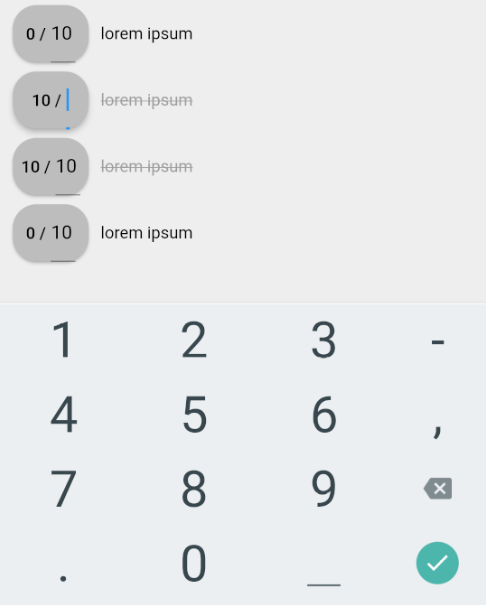
\includegraphics[width=6cm]{images/liczniki.png}
    \caption{Edycja celu jednego z liczników.}
    \vspace{3mm}
\end{figure}

\chapter{Implementacja}

Implementując aplikację MobiNote starałem się zachowywać czysty kod, podzielony na jak najmniejsze części pod względem odpowiedzialności i zadań klas oraz metod, jak również czyste repozytorium zachowując odpowiedni podział i strukturę katalogów, modułów i pozostałych plików. Przykładałem dużą wagę do jakości oraz wykonania, aby powrót do poszczególnych warstw i miejsc w aplikacji był prosty, a sama jej struktura była przejrzysta i zrozumiała. 

\section{Technologie}

\subsection{flutter}

Aplikacja została napisana przy użyciu frameworka flutter w języku Dart.

Wybierając technologie, kierowałem się kryteriami takimi jak: prostota, wieloplatformowość, estetyka bez dużego wkładu w kreowanie komponentów na własną rękę oraz wydajność. Jedną z najbardziej polecanych framework'ów na stronie \href{https://www.linkedin.com/pulse/best-9-mobile-app-development-frameworks-2023-sstech-system/}{linkedin.com} był \textbf{flutter}. Jak podaje strona główna \href{https://www.flutter.dev}{flutter.dev}:

"Flutter is an open source framework by Google for building beautiful, natively compiled, multi-platform applications from a single codebase."

Składnia języka Dart jest stosunkowo prosta i przejrzysta, natomiast framework Flutter pozwala na programowanie aplikacji mobilnych w prosty sposób na platformy IOS oraz Android o dużej wydajności zważywszy na to, że język Dart jest kompilowany do natywnego kodu. Pozwala to na tworzenie aplikacji szybko i bez wielkiego nakładu pracy, dając przy tym duże możliwości i przyjemny dla oka rozbudowany interfejs użytkownika.

%https://itcraftapps.com/pl/blog/flutter-w-swiecie-aplikacji-mobilnych-czy-to-przyszlosc-programowania/ 

\subsection{SQLite}

Do przechowywania notatek została wykorzystana baza danych SQLite. Aplikacja wykorzystuje bibliotekę \textbf{sqlite3}, umożliwiającą wykonywanie operacji na lokalnej bazie danych SQLite. Pozwala na ona na zapis, odczyt a także manipulację danymi. Dodatkowo wykorzystywany jest pakiet \href{https://pub.dev/packages/drift}{drift}, który jest rodzajem systemu ORM umożliwiającym mapowanie między obiektami języka Dart oraz tabelami bazy danych SQLite. Pozwala to na pracę bezpośrednio w kodzie Dart używając dostępnej funkcjonalności bez konieczności pisania zapytań bezpośrednio w języku SQL.

\section{Organizacja repozytorium}

Kod aplikacji został podzielony na moduły i zorganizowany w zależności od poziomu abstrakcji i zastosowań.

Główny katalog z kodem źródłowym \textbf{lib} zawiera:

\begin{itemize}
    \item plik \textbf{main.dart} z wywołaniem głównej funkcji main budującej aplikację,
    \item katalog \textbf{database}
    \item katalog \textbf{logic}
    \item katalog \textbf{screens}
\end{itemize}

\subsubsection{database}

Zawiera definicję bazy danych, struktury oraz metody z nią związane. Posiada wygenerowany na podstawie pliku \textbf{database\_{}def.dart} plik \textbf{database\_{}def.g.dart} zawierający struktury odzwierciedlające tabele bazy danych w klasy języka Dart. 

\subsubsection{logic}

Znajdują się tam definicje struktur reprezentujących stan komponentów, definicje typów (stylów tekstu, widgetów, znaczników itd.), mapowanie kluczy (String) na style tekstu, znaczniki i elementy, logika parsera, funkcje pomocnicze wraz z funkcjonalnością aplikacji niebędącej bezpośrednią częścią widgetów.

\subsubsection{screens}

Dostępne są tam definicje stron wraz z funkcjonalnością i metodami ich komponentów, jak również definicje motywów i kolorów aplikacji.

\section{Wykorzystane rozwiązania}

\subsubsection{Programowanie Obiektowe}

Dart promuje programowanie obiektowe, dlatego też w projekcie został zastosowany paradygmat obiektowego programowania wraz z jego mechanizmami. Przykładami tych mechanizmów może być wielokrotne zastosowanie abstrakcji różnych poziomów, dziedziczenie i polimorfizm.

Przykładem zastosowanie wszystkich powyższych mechanizmów jest reprezentowanie, tworzenie widgetów oraz zarządzania nimi. 
Dzięki zastosowaniu opisanych mechanizmów możliwe było zaimplementowanie fabryki, widgetów typu listy, oraz akapitów trzymanych w edytorze.

\subsubsection{Wzorce projektowe}

W powyższych opisach możemy zauważyć użycie niektórych wzorców projektowych spotykanych podczas pisania aplikacji mobilnej. Niektóre z nich opisane są na stronie \href{https://flutterdesignpatterns.com/}{flutterdesignpatterns.com}. Są to między innymi:

\begin{itemize}
    \item \textbf{Fabryka} -- użyty w przypadku fabryki widgetów \textit{NoteEditorWidgetFactory};
    \item \textbf{Singleton} -- używany w przypadku dostępu do bazy danych oraz dostępu do ustawionego motywu aplikacji (\textit{MobiNoteDatabase}, \textit{MobiNoteTheme});
    \item \textbf{Kompozyt} -- używany w przypadku struktur drzewiastych takich jak na przykład obiekty \textit{SpanTree}, czy \textit{NoteWidgetData};
\end{itemize}

\subsubsection{Testy Jednostkowe}

Część logiki niezwiązanej bezpośrednio z wyświetlaniem i organizacją komponentów i ich wyglądu testowałem za pomocą testów jednostkowych od razu podczas ich implementacji. Dzięki temu uniknąłem długich godzin poszukiwania problemów, gdy któryś z komponentów mógł nie działać poprawnie zważywszy na to, że problemem może być algorytm, jak i sam widget i funkcjonowanie frameworka flutter. Dostosowując szczegółowość testów jednostkowych starałem się pokryć przypadki użycia jeszcze przez użyciem danych klas, metod i algorytmów w aplikacji. Przetestowany został w ten sposób parser języka znaczników stylów, wraz z pełną funkcjonalnością, jak również konwersja reprezentacji widgetów do formatu JSON.

\subsection{Baza danych}

Do zarządzania dostępem i manipulacją bazy danych tworzony jest jeden obiektu typu \textbf{MobiNoteDatabase} dla całego projektu. Jest on tworzony i udostępniany za pomocą biblioteki do zarządzania stanem \textbf{GetX}. 

W implementacji aplikacji MobiNote, GetX pozwala na tworzenie instancji zarządzającej dostępem do bazy danych raz i udostępnianie jej w różnych miejscach aplikacji. Struktura aplikacji wymaga tylko jednej instancji obiektu MobiNoteDatabase, dlatego tworzone jest jedno połączenie w jej konstruktorze, a sam obiekt przechowywany jest z pomocą GetX

\begin{verbatim}
    Get.put(MobiNoteDatabase());
\end{verbatim}

\noindent Następnie za pomocą funkcji \textbf{find} może zostać udostępniany

\begin{verbatim}
    final database = Get.find<MobiNoteDatabase>();
\end{verbatim}

Umożliwia to zwiększenie wydajności, ponieważ unikamy otwierania połączenia z bazą danych za każdym razem, gdy jest ono potrzebne (obie strony: strona domowa, oraz edytor notatki używają połączenia z bazą danych do swoich funkcjonalności). Używany zatem jest tutaj wzorzec Singleton. Z racji tego, że nie ma potrzeby otwierania równoległych połączeń (używana jest tylko jedna ze stron i ich funkcjonalność naraz) wzorzec ten został zastosowany w implementacji.

\subsection{Dobre praktyki}

\subsubsection{Leniwe tworzenie widgetów w ListView}

Podczas implementacji listy notatek w stronie domowej oraz edytora zawartości notatki użyty został widget ListView poprzez wywołanie twz. \textit{named constructor} \textbf{ListView.builder}. Praktyka ta ma dobre zastosowanie przy długich listach, ponieważ używając konstruktora \textbf{builder} widgety zawarte w ListView budowane są w sposób leniwy, na bieżąco, jeśli istnieje potrzeba ich wyświetlenia. Z racji tego, że budowanie jest szybkie i nieskomplikowane pozwala to uniknąć przechowywania dużej ilości widgetów (znajduje to pozytywne skutki przy długich, skomplikowanych notatkach).
%https://docs.flutter.dev/cookbook/lists/long-lists

\subsubsection{Reprezentacja widgetów}

Każdy widget reprezentowany jest poprzez obiekt typu pochodnej klasy WidgetData przechowywującej parametry danego widgetu potrzebne do jego prawidłowego wyświetlania oraz funkcjonowania. Oddzielana jest warstwa wyświetlania od warstwy informacji danego widgetu. Pozwala to na zapis stanu widgetu do bazy danych, ponieważ zawarta w obiektach reprezentujących warstwę informacji jest funkcja konwersji do formatu JSON, który jest przechowywany w bazie danych jako fragment zawartości danej notatki.

\subsubsection{ID Generator}

Widgety zawierają identyfikatory do odróżniania ich w rodzicu lub liście zwierającej je. Ma to zastosowanie m.in. w znajdowaniu miejsca w liście np do dodawania nowego elementu, czy usuwania i zmiany elementów. Lepiej nadać id i na podstawie znalezienia id na liście pobierać index, zamiast nadawać i aktualizować indeksy za każdym razem elementom przy manipulacji listy.

Do generowania identyfikatorów w odpowiednich miejscach w kodzie służy obiekt klasy \textbf{IdGenerator}.

\subsubsection{Fabryka widgetów}

Widgety tworzone są na podstawie obiektów reprezentacyjnych(opisanych powyżej) w klasie \textbf{NoteEditorWidgetFactory}. Na podstawie pola \textbf{\textit{type}} wybierany jest typ widgetu, który następnie tworzony jest z parametrów obiektu reprezentującego. Używa klasy IdGenerator do generowania identyfikatorów, przez co obsługa przydzielania id jest robiona w jednym miejscu, w fabryce, która jest przekazywana dzieciom i elementom danych widgetów. Pozwala to zachować spójność w aktualnej implementacji, jak również przy dalszym rozwoju.

\chapter{Struktura Aplikacji}

Struktura aplikacji została częściowo opisana w rozdziale \hyperref[ch:manual]{\textbf{Podręcznik użytkownika}}.

\section{Edytor notatki}

Edytor notatki składa się z edytora tytułu znajdującego się w głównym pasku strony edycji notatki, oraz edytora zawartości.

\subsection{Zarządzanie zawartością}

Do zarządzania zawartością notatki używana jest klasa \textbf{NoteParagraphs} przechowująca listę obiektów typu \textbf{NoteParagraph} reprezentujących paragrafy notatki.
Współpracę tych klas można przedstawić w uproszczony sposób za pomocą schematu:

\begin{figure}[ht]
    \centering
    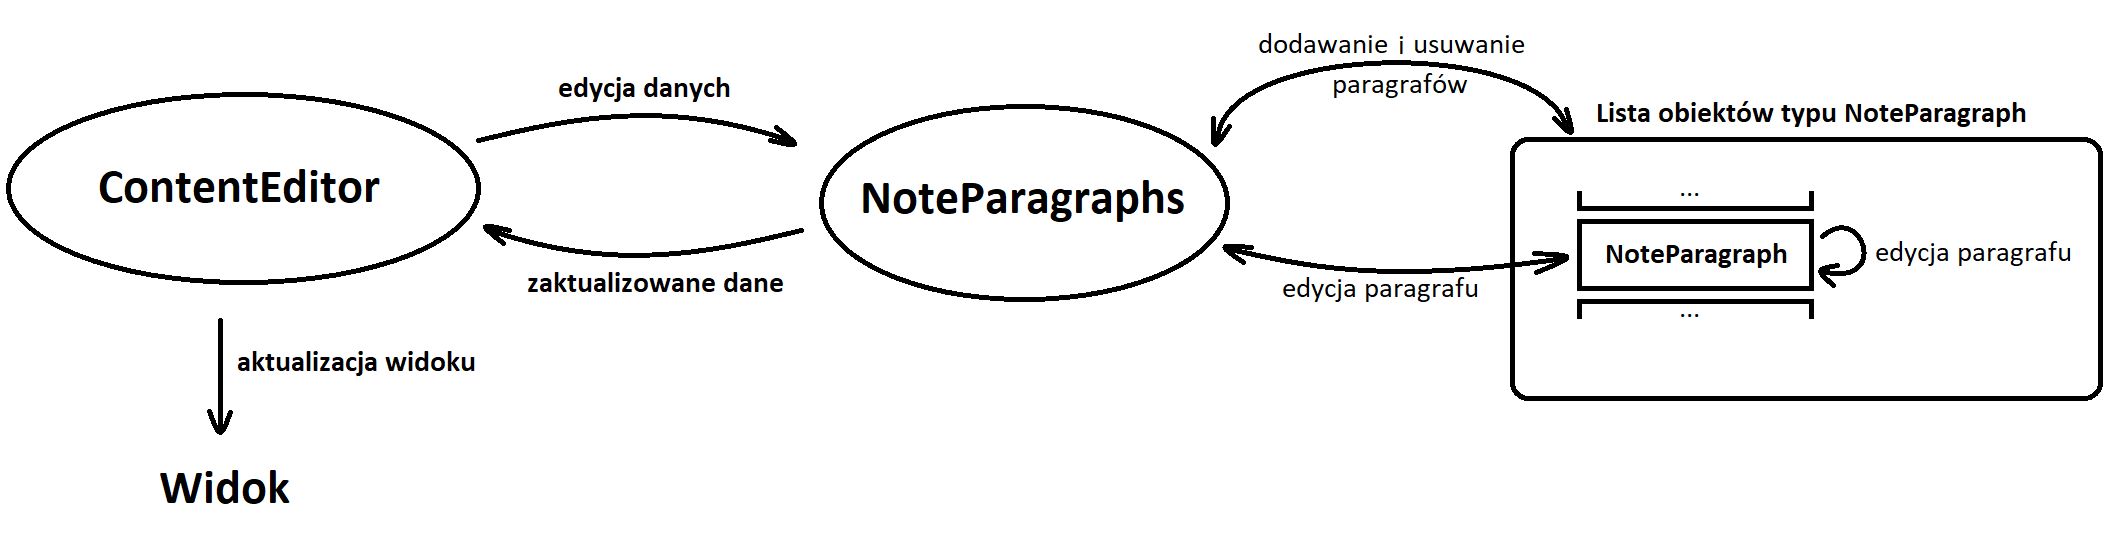
\includegraphics[width=\linewidth]{images/ContentEditor_podzial.png}
    \caption{Uproszczony schemat zarządzania paragrafami.}
\end{figure}

\newpage

\subsection{Paragrafy}

Istanieją trzy typy paragrafów w edytorze dziedziczące po \textbf{NoteParagraph}: 
\begin{itemize}
    \item \textbf{NoteParagraphTextEditor},
    \item \textbf{NoteParagraphWidget},
    \item \textbf{NoteParagraphPlaceholder}
\end{itemize}

Każdy z paragrafów posiada unikalny identyfikator \textbf{id} oraz referencję do fabryki widgetów tworzonej wewnątrz managera \textbf{NoteParagraphs}.
Pozwala to na unikalne identyfikowanie paragrafów wewnątrz listy, oraz wszystkich utworzonych widgetów w obrębie przestrzenii edytora.

Używane są również mechanizmy wywołań zwrotnych(callbacks) do zgłaszania aktywności(focus), zaistniałej zmiany, jak również usunięcia samego siebie z listy paragrafów, na podstawie swojego id, gdy wszystkie jego elementy zostaną usunięte.

\subsubsection{NoteParagraphTextEditor}

Służy do przechowywania, wyświetlania i edycji tekstu notatki. Posiada mechanizmy dynamicznej zmiany rozmiaru poprzez manipulację stanem oraz wartościami wewnętrznych pól. Posiada tylko jeden element, którym jest pole tekstowe z niestandardowym kontrolerem parsującym tekst przy użyciu własnego parsera.

\subsubsection{NoteParagraphWidget}

Służy do przechowywania, wyświetlania i edycji widgetów notatki. Posiada mechanizmy dynamicznej zmiany rozmiaru wraz ze zmianą rozmiaru widgetu będącego elementem głównym. Mechanizmy zmiany rozmiaru są różne w zależności od rodzaju widgetu.

\subsubsection{NoteParagraphPlaceholder}

Służy jako wypełnienie pozostałej przestrzeni edytora. Po kliknięciu na niego uruchamia mechanizm przenoszenia aktywności(focus) na ostatni paragraf na liście, dzięki czemu użytkownik nie musi znać wielkości i szukać ostatniego paragrafu, aby kontynuować edycję notatki.

\section{Praca z tekstem}

Praca z tekstem dzieli się na edycję tekstu z użyciem logiki zawartej w \textbf{NoteParagraphTextEditor}, jak również wyświetlanie go wraz ze zmianą rozmiarów z pomocą \textbf{NoteTextEditingController}.

\subsection{Edycja Tekstu}

Tekst edytowany jest za pomocą pola tekstowego TextField udostępnianego jako widget przez framework flutter. Posiada on wewnętrzny padding poziomy(lewa i prawa strona) jako stałą wartość, oraz padding pionowy(góra, dół) obliczany na podstawie różnicy pomiędzy wielkoścą czcionki użytej w danym paragrafie, a domyślnej czcionki z dodatkiem podstawowej wartości niezerowej(w przypadku, gdy dany paragraf nie ma ustawionego nagłówka, nie chcemy braku odstępu między paragrafami z powodu zerowego paddingu pionowego).

Przy każdej zmianie tekstu sprawdzana jest jego zawartość w poszukiwaniu informacji o stanie paragrafu. Stan ten określa się poprzez wielkośc czcionki i stylów tekstu użytych w paragrafie.

\subsubsection{Dodawanie tekstu}

Jeśli wewnątrz pola tekstowego został dodany znak nowej linii, wówczas wołane jest wywołanie zwrotne(callback), zainicjalizowane przy tworzeniu danego paragrafu przez \textbf{NoteParagraphs}, do dodawania nowego paragrafu. Wywołanie to przyjmuje identyfikator danego paragrafu i na tej podstawie oblicza miejsce w liście do którego należy włożyć nowopowstały paragraf. Przy tworzeniu nowego paragrafu następuje przeniesienie tekstu następującego po znaku końca linii. Znak końca linii jest usuwany.

\subsubsection{Usuwanie tekstu}
\label{eq:usuwanieTekstu}

Flutter nie oferuje możliwości przechwycenia zdarzenia naciśnięcia przycisku \textbf{delete}, gdy kursor znajduje się na początku tekstu. W tej sytuacji najprościej jest użyć przechwycenia zdarzenia edycji tekstu w paragrafie.

W każdym paragrafie na początku dodawany jest znak \verb|placeholder = \u200b|. Jest to znak unicode reprezentujący spację o zerowej długości, a więc niewidoczną w tekście. Jest to swego rodzaju wartownik, którego brak na początku tekstu podczas sprawdzania tekstu po edycji, mówi o potrzebie usunięcia paragrafu.

Gdy użytkownik zechce usunąć paragraf, wówczas przenosi się kliknięciem na początek wiersza(o ile już się na nim nie znajduje), a następnie naciska przycisk \textbf{delete}. Dzięki temu usuwa \verb|placeholder|, a przy tym wywoływany jest callback służący do usunięcia paragrafu. Jako argument przyjmuje identyfikator paragrafu, aby określić miejsce usunięcia.

Aby uniknąć kliknięcia na początek linii, przed wartownika, dodany został mechanizm zmiany pozycji kursora na drugi znak(bezpośrednio za wartownikiem) za każdym razem gdy jest on na pozycji zerowej.

\subsection{Wyświetlanie tesktu}

Do wyświetlania stylizowanego tekstu używane są obiekty typu \textbf{TextSpan}. Obiekty te posiadają drzewiastą strukturę, ponieważ mogą zawierać dzieci tego samego typu, które będą dziedziczyć dane parametry stylu, o ile nie zostaną dla nich specjalnie zainicjalizowane. Daje to możliwość zorganizowania tesktu bez potrzeby dzielenia go na małe kawałki oraz nadawania za każdym razem łączonych styli(gdyby obiekty \textbf{TextSpan} były przechowywane jako elementy jednej listy). Można zainicjalizować jeden styl wewnątrz drugiego, co bardzo upraszcza strukturę i pozwala na wprowadzanie globalnych zmian struktury(jak na przykład wielkość czcionki całego paragrafu) tylko w korzeniu, zapewniając, że wszystkie części tekstu odziedziczą zmianę.

Aktualizacja i renderowanie wyglądu pola tekstowego na bieżąco jest możliwe poprzez wykorzystanie klasy \textbf{TextEditingController}. Posiada ona metodę \textbf{buildTextSpan}, która służy do budowania wyglądu i stylu tekstu poprzez obiekty \textbf{TextSpan}. Dzieczicząc z tej klasy i nadpisując metodę \textbf{buildTextSpan} mogłem użyć parsera tekstu zawierającego znaczniki do przekonwertowania go na stylizowany tekst.
Dzięki temu przy każdej zmianie tekst jest parsowany, a jego wygląd aktualizowany.

Utworzony w ten sposób \textbf{NoteTextEditingController} może nie tylko używać parsera do tworzenia obiektów \textbf{TextSpan}, ale również mógł zostać rozszerzony o dodatkowe parametry, takie jak:

\begin{compactitem}
    \item callback \textbf{resizeTextField} wołany podczas parsowania, gdy wielkość czcionki w tekście ulega zmianie, 
    \item możliwość przechowywania informacji o tym, czy dany paragraf jest aktualnie w użyciu,
    \item sprawdzanie i manipulacja pozycją kursora.
\end{compactitem}

Callback \textbf{resizeTextField} został użyty w kontrolerze, zamiast w widgecie pola tekstowego, ponieważ wtedy wystarczy parsować tekst jednokrotnie. Przed samym zwróceniem drzewiastej struktury tekstu \textbf{TextSpan} możemy ustawić rozmiar pola tekstowego w jego korzeniu, zamiast edytować zawartość widgetu w innych mechanizmach i tak czy inaczej parsować dodatkowo tekst w poszukiwaniu informacji na temat wielkości czcionki.

Informacja na temat aktualnego użycia paragrafu jest używana do wyświetlania i ukrywania znaczników stylu nagłówka.

Sprawdzanie i manipulacja pozycją kursora pozwala na odkrywanie znaczników stylu, jak również ustawianie pozycji, aby kursor nie znajdował się przed znakiem \verb|placeholder|(zobacz \hyperref[eq:usuwanieTekstu]{Usuwanie tekstu}).

Przy każdej zmianie tekstu odświeżany jest widok paragrafu, dlatego wystarczy zmienić wartość zmiennej odpowiadającej za jego rozmiar przed końcem całej operacji związanej z przetwarzaniem nowego tekstu.
%https://api.flutter.dev/flutter/widgets/TextEditingController/buildTextSpan.html

\subsection{Problem parsowania tekstu ze znacznikami stylu}

Do wyświetlania stylizowanego tekstu potrzebne jest jego parswoanie. Funkcjonalnośc ta, będzie wołana stosunkowo często, a dla długich tekstów bez znaku nowej linii będzie to długi do obsługi tekst. Dlatego też ważny jest sposób implementacji.

Zrealizowanym pomysłem rozwiązania problemu jest podział parsowania tekstu na trzy etapy:
\begin{enumerate}
    \setlength\itemsep{0mm}
    \item przkształcanie znaczników stylu w tekście na \textbf{znaki unicode}
    \item parsowanie tekstu ze \textbf{znakami unicode} na specjalną drzewiastą reprezentację \textbf{SpanInfo}
    \item konwersja struktury \textbf{SpanInfo} na obiekt \textbf{TextSpan}
\end{enumerate}

\subsection{Implementacja Parsera}

\subsubsection{Własna implementacja}

Parser wraz z jego strukturą został zaprojektowany i zaimplementowany przeze mnie, zamiast przy użyciu narzędzi generowania parsera dla opisanej gramatyki użwanego przeze mnie języka znaczników. Powodem tego jest potrzeba łatwego rozwoju oraz wprowadzenia niestandardowych rozwiązań i dodatkowych funkcjonalności niebędących częścią samej składni gramatyki, jednak potrzebnych wewnątrz implementacji parsera.

Własna implementacja parsera pozwoliła mi od początku do końca zaprojektować i zrozumieć jego strukturę dzięki czemu przykładowo wprowadzanie funkcji odkrywania i ukrywania znaczników stylu oraz nagłówka, bądź dodanie wywołania zwrotnego zmieniającego rozmiar pola tekstowego, było prostym zabiegiem niewymagającym dużych zmian i rozrzerzeń kodu parsera.

\subsubsection{Parsowanie}

Każdy z etapów parsowania jest realizowany poprzez inną klasę. Całość łączona jest w metodzie obiektu \textbf{NoteTextEditingController}.
\newline
\begin{figure}[ht]
    \centering
    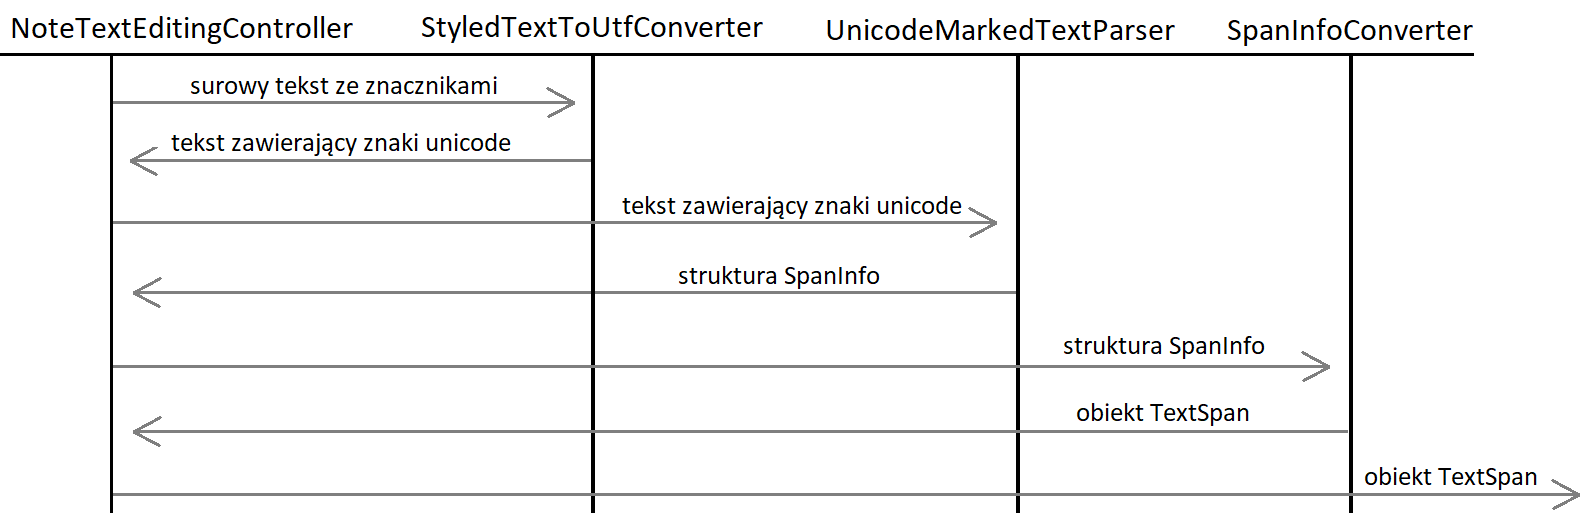
\includegraphics[width=\linewidth]{images/etapy_parsowania.png}
    \caption{Schemat przedstawiający etapy parsowania tekstu.}
    \label{fig:etapyParsowania}
\end{figure}

\subsubsection{Znaki unicode}

%https://unicode.org/glossary/#private_use_area
Do procesu parsowania zostały użyte znaki unicode z bloku Private Use Area(Prywatny Obszar Użytkowania). Są to znaki, które są trudno dostępne dla użytkownika z poziomu klawiatury mobilnej.

\noindent Zdefiniowane zostały w następujący sposób:

\begin{lstlisting}[language=java]
const styleUnicodeNumber = 0xe000;
const widgetUnicodeNumber = 0xe100;
const elementUnicodeNumber = 0xe1A0;
const paragraphUnicodeNumber = 0xe200;
\end{lstlisting}

Oznaczają odpowiednio początki przestrzeni znaczników: stylu tekstu, wewnętrznych widgetów i elementów w tekście oraz nagłówków paragrafu.
Znaczniki początkowe mają parzyste numery, natomiast znaczniki końcowe mają nieparzyste numery następujące po odpowiadających im znacznikach początkowych.

\subsubsection{Struktura SpanInfo}

Podczas implementacji użyta została struktura \textbf{SpanInfo}. Zawiera ona informacje na temat danego węzła w drzewiastej strukturze stylów tekstu, oraz referencję do jego rodzica.
Została zaimplementowana w celu usprawnienia przebiegu etapu drugiego parsowania tekstu.

\begin{lstlisting}[language=java]
class SpanInfo {
  String type;
  String text;
  List<SpanInfo> children;
  late SpanInfo parent;
}
\end{lstlisting}

Dzięki swojej budowie struktura może zostać przekonwertowana w prosty sposób na obiekt typu \textbf{TextSpan}.

\subsubsection{StyledTextToUtfConverter}

Przekształcanie znaczników odbywa się poprzez przejście przez tekst w ich poszukiwaniu i przetwarzaniu. Znaczniki dzielone są na początkowe i końcowe(zobacz: \hyperref[subsec:ustawianieStyli]{Ustawianie styli}). Podczas sprawdzania czy dany znak jest znacznikiem początkowym, czy końcowym pobierany jest szerszy kontekst, złożony z przylegających do niego znaków.

W momencie, gdy zostanie znaleziony znak będący początkowym znacznikiem, dodawana jest informacja o nim do listy \textbf{startBounds} w postaci struktury \textbf{SpecialPatternInfo} przechowującej znacznik wraz z jego indeksem.

\begin{lstlisting}[language=Java]
class SpecialPatternInfo {
  final int indexInText;
  final String character;
}
\end{lstlisting}

W przypadku znalezienia znaku $c$ będącego końcowym znacznikiem, przeszukujemy listę \textbf{startBounds} w poszukiwaniu pierwszego wystąpienia znacznika $c'$ o takiej samej wartości. Jeśli nie zostanie znaleziony, wówczas znak $c$ traktowany jest jako zwykły tekst. Jesli natomiast zostanie znaleziony, oznacza to, że wystąpił wcześniej początek stylu, a cały tekst pomiędzy aktualnym indeksem, a indeksem zapisanym w strukturze opisującej początkowy znacznik $c'$ jest tekstem zawierającym ten styl. Zatem znalezione znaczniki zamieniane są na swoje odpowiedniki w formie znaków unicode, a znaczniki istniejące na liście będące następnikami znalezionego $c'$ zostają usunięte z listy(style nie mogą się przecinać), a więc nie zostaną zamienione.

W podobny sposób konwertowane są również widgety i elementy wewnętrzne w tekście. W aktualnej wersji aplikacji nie są one obsługiwane, jednak sam parser został przygotowany na obsługę tego typu problemu. Szukane są zatem również fragmenty tekstu będące tagami widgetów bądź oznaczeniami elementów.

\subsubsection{UnicodeMarkedTextParser}

Z racji tego, ze znaki unicode z tego zakresu są trudno dostępne, na potrzeby samego problemu konwersji tekstu notatek możemy założyć, że znaki w tekście symbolizują początkowe i końcowe znaczniki, które na pewno mają swoje odpowiedniki i są poprawnie użyte(nie przecinają się).

Na początku algorytmu tworzona jest referencja $currentSpan$ na obiekt \textbf{SpanInfo}, który jest aktualnie przetwarzanym stylem(napotkany został jego znacznik początkowy). Początkowo jest to korzeń całej struktury \textbf{SpanInfo}.

Oznaczony w ten sposób tekst przechodzimy ponownie, jednak posiadając dokładne informacje, które symbole są znacznikami stylu, a które zwykłymi fragmentami tekstu.

Podczas przechodzenia tekstu zapisujemy znaki niebędące znacznikami do tymczasowego bufora.

Napotykając znacznik początkowy, jeśli w buforze znajduje się tekst, to wówczas jest on dodawany do tekstu przechowywanego w $currentSpan$. Następnie tworzony jest nowy \textbf{SpanInfo}, na podstawie stylu reprezentowanego przez znacznik, będący dzieckiem $surrentSpan$ i zapisywany jest jako $currentSpan$. 

Po napotkaniu znacznika końcowego dodajemy tekst z tymczasowego bufora do $currentSpan$, czyścimy bufor i przestawiamy $currentSpan$ przechodząc po węzłach \textbf{SpanInfo}(używane jest do tego pole z referencją $parent$ wskazującą na rodzica danego węzła) na pierwszy napotkany węzeł przechowujący informacje na temat stylu reprezentowanego przez aktualnie sprawdzany znacznik.

Przetwarzane są również informacje na temat widgetów i elementów wewnętrznych przygotowane w ramach podstawy do rozwoju funkcjonalności w przyszłosci.

\subsubsection{SpanInfoConverter}

Klasa \textbf{TextSpan} jest klasą pochodną klasy \textbf{InlineSpan}.

\textbf{SpanInfoConverter} buduje strukturę \textbf{InlineSpan} złożoną z obiektów klas pochodnych \textbf{TextSpan} oraz \textbf{WidgetSpan}. Biorąc pod uwagę, że wewnętrzne widgety i elementy, które mają w przyszłości być obsługiwane przy użyciu \textbf{WidgetSpan} nie są aktualnie obsługiwane przyjęty w opisie model struktury opiera się tylko na obiektach typu \textbf{TextSpan}.

Przechodząc przez strukturę \textbf{SpanInfo} budujemy strukturę złożoną z obiektów typu \textbf{TextSpan}. Zapisywany jest $mainSpan$ będący korzeniem struktury, natomiast przejście przez strukturę odbywa się w sposób rekurencyjny.

\begin{lstlisting}[language=Java]
SpanInfo mainSpan = SpanInfo(type: 'null');

InlineSpan getSpans(SpanInfo spanInfo) {
    if (mainSpan.type == 'null') mainSpan = spanInfo;

    List<InlineSpan> spanChildren =
        spanInfo.children.map((e) => getSpans(e)).toList();

    /* ustawianie stylu i typu obiektu 
     * oraz zwracanie go wraz z children */
}
\end{lstlisting}





\chapter{Rozwój Aplikacji}

\section{Struktura Aplikacji}

\subsection{Baza danych}

\subsection{Strona główna}

\subsection{Edytor notatek}

\subsection{Dodatkowe strony}

\section{Rozszerzenie istniejących rozwiązań}

\subsubsection{Lista}

Klasa \textbf{NoteElementListWidget} posiada zmienną \verb|int depth| służącą do określania poziomu głębokości w liście. Ma to na celu określenie wielkości wcięcia, jak również uzywanych etykiet do oznaczania danego elementu(różne znaki, numeracja itd).

Dodatkowym elmenetem do edycji listy jest możliwość własnej definicji etykiet w liście. Będzie to ograniczone do pewnej głębokości. W zależności od głębokości, użytkownik będzie mógł zdefiniować symbol lub napis, który będzie używany jako etykieta.

\subsection{Widgety wewnętrzne w tekście}

Aktualnie w kodzie przygotowane są miejsca do parsowania widgetów wewnętrznych w tekście. Przygotowane są definicje wzorów w tekście, które miałyby zostać przekonwertowane w widgety.

Widgetami wewnętrzymi są między innymi:

\begin{compactitem}
    \item linki stron internetowych
    \item linki notatek w bazie
    \item inline latex -- do dodawania na przykład symboli matematycznych
    \item zdjęcia (o rozmiarze nieprzekraczającym rozmiaru czcionki)
    \item cytowanie tekstu(zmiana koloru tła tekstu oraz czcionki)
\end{compactitem}

Użycie obiektów \textbf{InlineSpan} udostępnianych przez flutter pozwala tworzyć drzewiastą strukturę, której korzeniem jest \textbf{TextSpan}, natmiast dziećmi są inne obiekty \textbf{InlineSpan}, czyli instancje obiektów klas pochodnych \textbf{TextSpan} i \textbf{WidgetSpan}.
%https://api.flutter.dev/flutter/painting/InlineSpan-class.html

\subsection{Dodatkowe Widgety w notatce}

Przygotowane również zostały obiekty typu \textbf{NoteWidgetData} oraz miejsca w \textbf{NoteListElementWidget} na dodatkowe elementy takie jak na przykład \textbf{NoteInfoPage}, która będzie widgetem złożonym z ikony, który po kliknięciu otwiera okno dialogowe ze przewijalną notatką/stroną informacyjną.

Planowanymi dodatkowymi widgetami są między innymi:

\begin{compactitem}
    \item notatka głosowa(zobacz \hyperlink{sec:glosowaNotatka}{Nagrywanie głosowej notatki}
    \item 
\end{compactitem}

\subsection{Interakcja widgetów}

\section{Funkcjonalność}

\subsection{Alarmy}

\subsection{Powiadomienia}

\subsection{Nagrywanie głosowej notatki}
\label{sec:glosowaNotatka}

\subsection{Karty Step-By-Step}



%%%%% BIBLIOGRAFIA

\begin{thebibliography}{1}
\bibitem{googleplay} 
Opis platformy Google Play dostępny na stronie \url{https://play.google/howplayworks/}

\bibitem{linkedin}
SSTech System on linkedin.com (15.03.2023) \emph{BEST 9 MOBILE APP DEVELOPMENT FRAMEWORKS IN 2023}, \url{https://www.linkedin.com/pulse/best-9-mobile-app-development-frameworks-2023-sstech-system/}

\bibitem{itCraft}
itCraft (26.05.2023) \emph{Flutter w świecie aplikacji mobilnych: Czy to przyszłość programowania?}, \url{https://itcraftapps.com/pl/blog/flutter-w-swiecie-aplikacji-mobilnych-czy-to-przyszlosc-programowania/}

\bibitem{flutter}
Opis oraz dokumentacja frameworka flutter: \url{https://www.flutter.dev}

\bibitem{sqlite3}
Opis biblioteki sqlite3 dla języka Dart: \url{https://pub.dev/packages/sqlite3}

\bibitem{drift}
Opis biblioteki drift dla języka Dart: \url{https://pub.dev/packages/drift}, dokumentacja: \url{https://drift.simonbinder.eu/docs/getting-started/}

\bibitem{flutterdesignpatterns}
Wzorce projektowe spotykane podczas implementacji aplikacji mobilnych z użyciem frameworka flutter opisane zostały na stronie: \url{https://flutterdesignpatterns.com/}

\end{thebibliography}

\end{document}